\begin{figure}[tb]
    \centering
    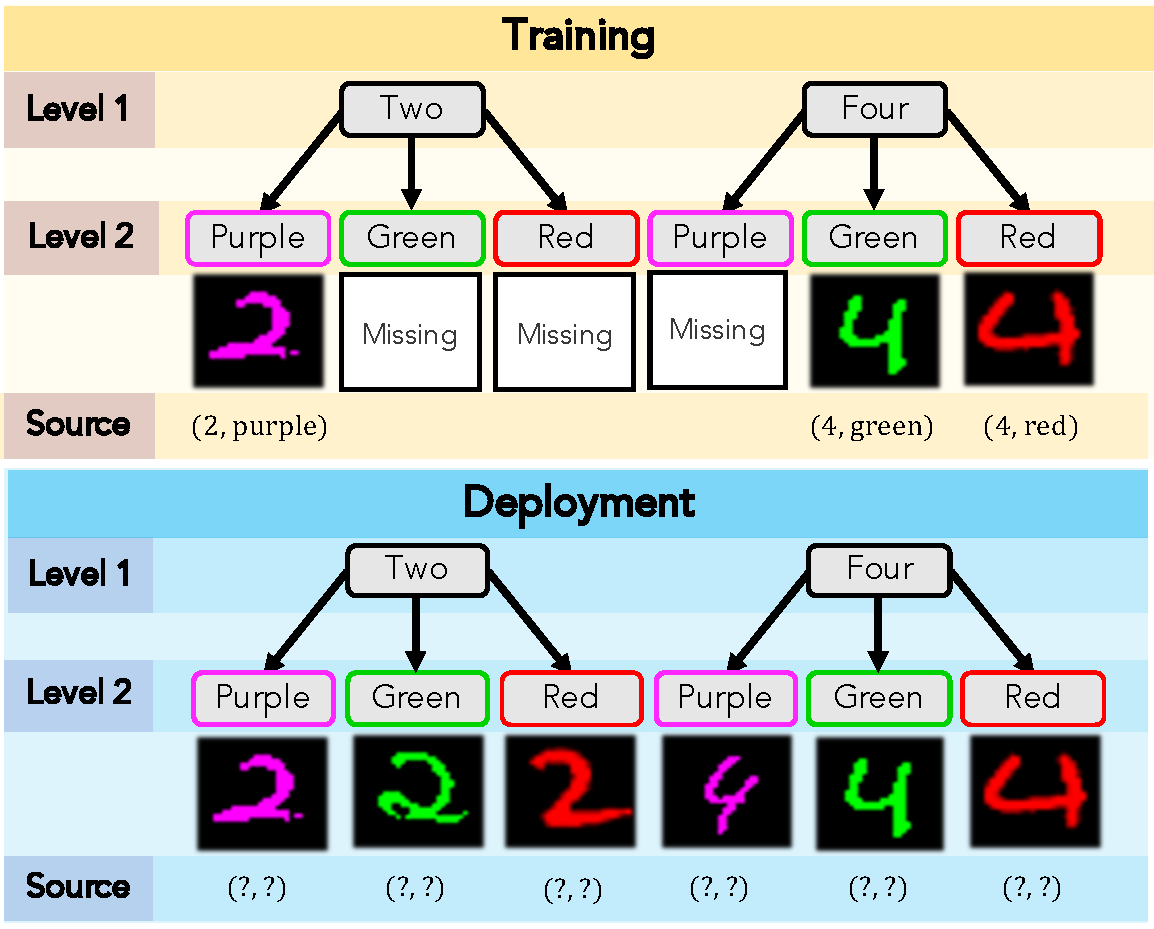
\includegraphics[width=0.7\columnwidth]{supmatch/figures/illustrations/problem_setup.pdf}
    \caption{%
      Illustration of our general problem setup. 
      %
      We assume the data follows a two-level hierarchy in which the first level corresponds to the class-level information (digit) and the second level corresponds to subgroup-level information (color).
      %
      While all digits appear in the training set (Top), not all digit-color combinations (sources) do; these gaps in conditional support give rise to a spurious correlation between digit and color, where the former is completely determined by the latter in the training set (giving the mappings $\textrm{{\color{purple}purple}} \rightarrow \texttt{2}$ and $\textrm{{\color{green}green}} \lor \textrm{{\color{red}red}} \rightarrow \texttt{4}$ as degenerate solutions to the classification problem), yet this same correlation does not hold for the deployment set (Bottom) which contains samples from the missing combinations.
      %
      To disentangle the (spurious) subgroup- and class-related information, we make use of an additional dataset that is representative of the data the model is expected to encounter at deployment time, in terms of the sources present.
    }%
    \label{fig:problem-setup}
\end{figure}


Machine learning has burgeoned in the last decade, showing the ability to solve a wide variety of
tasks with unprecedented accuracy and efficiency.
%
These tasks range from image classification \citep{krizhevsky2012imagenet} and object detection
\citep{ren2015faster}, to recommender systems \citep{ying2018graph} and the modelling of complex
physical systems such as precipitation \citep{ravuri2021skillful} and protein folding
\citep{jumper2021highly}.
%
In the shadow of this success, however, one finds less cause for optimism in frequent failure in
equitability and generalisation-capability, failure which can have serious repercussions in
high-stakes applications such as self-driving cars \citep{sun2019unsupervised}, judicial
decision-making \citep{mayson2018bias}, and medical diagnoses \citep{albadawy2018deep}.
%
ML's data-driven nature is a double-edged sword: while it opens up the ability to learn patterns
that are infeasibly complex for a practitioner to encode by hand, the quality of the solutions
learned by these models depends primarily on the quality of the data with which they were trained.
%
If the practitioner does not properly account for this, models ingesting data ridden with biases
will assimilate, and sometimes even amplify, those biases.
%
The problem boils down to not having sufficiently diverse annotated data, however collecting more
labelled data is not always feasible due to temporal, monetary, legal, regulatory, or physical
constraints.

%
While data can be intrinsically biased (such as in the case of bail records),
\emph{representational bias} is more often to blame, where socioeconomic or regulatory factors
resulting in certain demographics being under- (or even un-) represented. 
%
Clinical datasets are particularly problematic for ML due to the frequency of the different
outcomes being naturally highly imbalanced, with the number of negative cases (\texttt{healthy})
typically greatly outweighing the number of positive cases (\texttt{diseased}); even if a subgroup
is well-represented overall, that may well not be the case when conditioned on the outcome.
%
Equally, it is entirely possible that certain subgroups may be completely absent. 
%
For example, pregnant women are often excluded from clinical trials due to safety concerns, and if
they do participate it is often at too low a rate to be meaningful \citep{afrose2021overcoming}.

Like many prior works
\citep{SohDunAngGuetal20,kim2019learning,creager2021environment,SagRagKohLia20}, we consider
settings where there is a two-level hierarchy, with the second level partitioning the data into
\emph{subgroups} that are causally independent of the class (constituting the first level) which is
being predicted. 
%
This second level of the data is assumed to be predictable by the classifiers in the considered
hypothesis class. 
%
In both \citet{SohDunAngGuetal20} and \citet{creager2019flexibly} the entailed subgroups are
unobserved and need to be inferred in a semi-supervised fashion. We consider a similar problem but
one where the second level is partially observed.
%
Specifically, we focus on problems where some outcomes are available for some subgroups and not for
others. 
%
This particular form of the problem has -- so far as we are aware -- been hitherto overlooked
despite pertaining to a number of real-world problems.

%
If the labelled training set is sufficiently balanced in terms of classes and subgroups, a standard
ERM (empirical risk minimisation) classifier can achieve good performance.
%
However, we consider the added difficulty that, in the labelled training set, some outcomes
(classes) are not observed for all subgroups, meaning some of the classes do not overlap with all
the subgroups.
%
In other words, in the training set, some of the classes have \emph{incomplete support} with
respect to the subgroup partition, while in the deployment setting we expect all possible
combinations of subgroup and class to appear.
%
We illustrate our problem setup in Fig.~\ref{fig:problem-setup}, using Coloured MNIST digits as
examples; here, the first level of the hierarchy captures digit class, the second level, colour. 
%
While the (unlabelled) deployment set contains all digit-colour combinations (or \emph{sources}),
half of these combinations are missing from the (labelled) training set. 
%
A classifier trained using only this labelled data would wrongly learn to classify \texttt{2}s based
on their being {\color{purple}purple} and \texttt{4}s, based on their being {\color{green}green} or
{\color{red}red} (instead of based on shape) and when deployed would perform no better than random
due to the new sources being coloured contrary to their class (relative to the training set).

We address this problem by learning representations that are invariant to subgroups and that thus
enable the model to ignore the subgroup partition and to predict only the class labels.
%
In order to train an encoder capable of producing these representations, the information contained
in the labelled training set alone is not sufficient to break the \emph{spurious correlations}.
%
To learn the ``correct'' representations, we make use of an additional unlabelled dataset with
support equivalent to that of the deployment set (which includes the possibility of it being the
actual deployment set).
%
We do not consider this a significant drawback as such data is almost always far cheaper and less
labour-intensive to procure than \emph{labelled} data (which may require expert knowledge).
%

This additional dataset serves as the inductive bias needed by the encoder to disentangle class-
and subgroup-related factors.
%such that a downstream predictor can be trained using the available labels without risk of
%internalizing the spurious correlations present in the original data.
%
The encoder is trained adversarially to produce representations whose source (\texttt{training} or
\texttt{deployment}) is indeterminable to a set-classifier.
%
To ensure subgroup- (not class-) invariance is learned, the batches fed to the discriminator need
to be approximately balanced, such that they reflect the support, and not the shape, of the
distributions. 
%
We propose a practical way of achieving this based on semi-supervised clustering.
%

We empirically show that our proposed method can effectively disentangle subgroup and semantic
factors on a range of classification datasets and is robust to noise in the bag-balancing, to the
degree of outperforming the baseline methods even when no balancing of bags from the deployment set
is performed.
%
Furthermore, we prove that the entailed objective is theoretically guaranteed to yield
representations that are invariant to subgroups and that we can bound the error incurred due to
imperfect clustering.

